\chapter{Ocena działania algorytmu}
Na przygotowanym systemie przeprowadzone zostały badania reakcji systemu na ruch drogowy o przepływach przedstawionych na rysunku \ref{fig:mapa_ruch}. Każda konfiguracja była badana przez jedną godzinę, a wielkości badane to: średnia liczba zatrzymań wszystkich pojazdów, średnia prędkość wszystkich pojazdów oraz średnie czasy przejazdu na trzech, wybranych, trasach, przedstawionych na rysunku \ref{fig:mapa_trasy}.

\section{Wyniki badań}
W tabeli \ref{tab:predkosc} przedstawione zostały wartości średniej liczby zatrzymań i średniej prędkości w zależności od typu i parametrów sterowania.

\FloatBarrier
\begin{table}[h]
	\centering
	\begin{tabular}{ |r|c|c| }
		\hline
		& średnia liczba zatrzymań & średnia prędkość \\
		\hline
		brak kontroli                             & 33,01 & 12,02 km/h \\
		\hline
		stałoczasowa                              & 16,57 &  6,35 km/h \\
		\hline
		dynamiczna, 60s, p=0,33, q=0,33, r=0,33   & 11,00 &  9,32 km/h \\
		\hline
		dynamiczna, 90s, p=0,33, q=0,33, r=0,33   &  9,39 &  9,68 km/h \\
		\hline
		dynamiczna, 120s, p=0,33, q=0,33, r=0,33  &  8,30 &  9,70 km/h \\
		\hline
		dynamiczna, 120s, p=0,5, q=0,25, r=0,25   &  8,32 &  9,17 km/h \\
		\hline
		dynamiczna, 120s, p=0,8, q=0,1, r=0,1     &  8,38 &  9,15 km/h \\
		\hline
		dynamiczna, 120s, p=0,25, q=0,5, r=0,25   &  8,29 &  9,73 km/h \\
		\hline
		dynamiczna, 120s, p=0,1, q=0,8, r=0,1     & 11,54 &  8,85 km/h \\
		\hline
		dynamiczna, 120s, p=0,25, q=0,25, r=0,5   &  9,45 &  9,34 km/h \\
		\hline
		dynamiczna, 120s, p=0,1, q=0,1, r=0,8     & 10,72 &  9,35 km/h \\
		\hline
	\end{tabular}
	\caption{Zależność średniej liczby zatrzymań i średniej prędkości od typu i parametrów sterowania}
	\label{tab:predkosc}
\end{table}
\FloatBarrier
\begin{figure}[h]
    \centering
    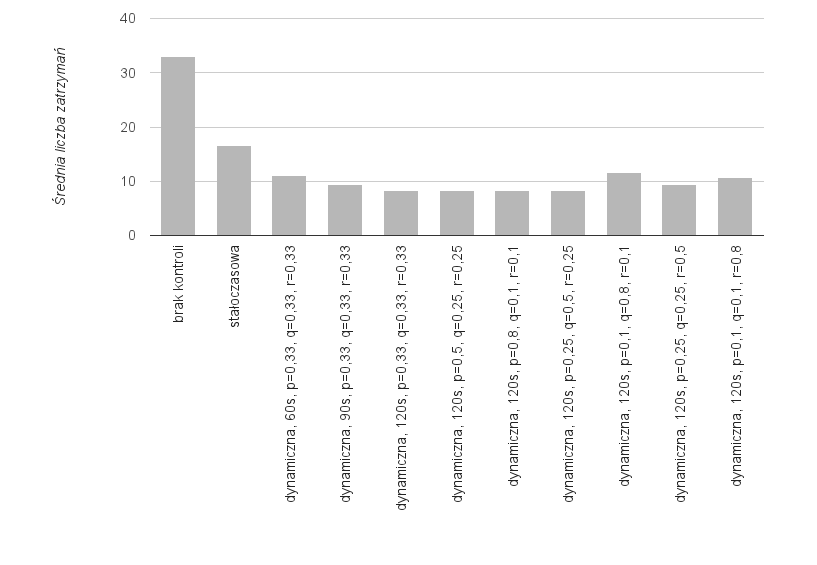
\includegraphics[width=1.0\textwidth]{images/wykres_liczba_zatrzyman.png}
    \caption{Wykres zależności średniej liczby zatrzymań od typu i parametrów sterowania}
    \label{fig:wykres_liczba_zatrzyman}
\end{figure}
\FloatBarrier

Na wykresie średniej liczby zatrzymań (rys. \ref{fig:wykres_liczba_zatrzyman}) możemy zaobserwować podstawową różnicę charakterystyki ruchu sterowanego i nie sterowanego.
Niekontrolowany ruch wykazuje się dużą, w porównaniu z pozostałymi badanymi konfiguracjami, liczbą zatrzymań co może być spowodowane ruchem krokowym ruchem pojazdów czekających na przejazd, na przykład wyjeżdżających z ulicy podporządkowanej. Jest to analogiczne z ruchem pojazdów poruszających się w korku i często przejeżdżającymi zaledwie kilka metrów.

Badany algorytm dynamiczny charakteryzuje się również lepszą, mniejszą, liczbą zatrzymań pojazdów niż stałoczasowy program sygnalizacji.
Spośród badanych wartości parametrów, najlepsza wydaje się konfiguracja podstawowa, o równej wielkości badanych parametrów, oraz konfiguracja faworyzująca spodziewany przepływ pojazdów otrzymany od sąsiadujących kontrolerów. Większa długość cyklu uzyskuje lepsze wyniki ze względu na rzadszą, wymuszoną, zmianę świateł.

\FloatBarrier
\begin{figure}[h]
    \centering
    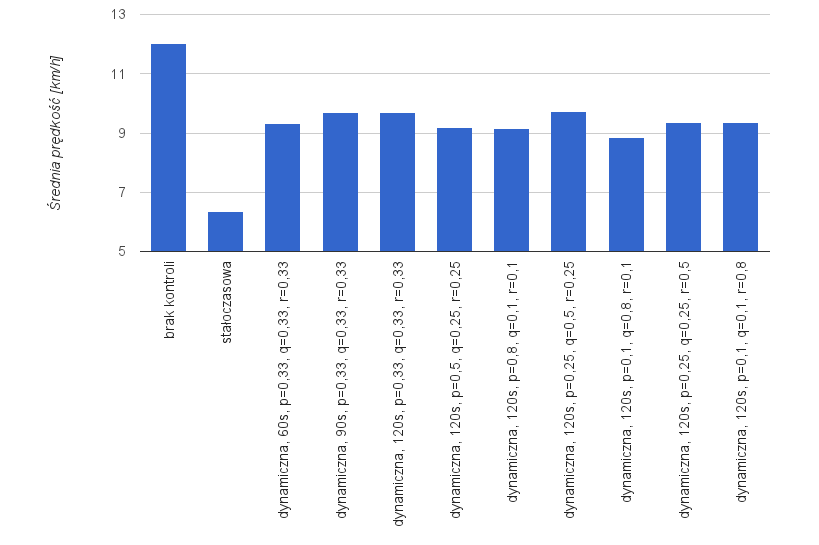
\includegraphics[width=1.0\textwidth]{images/wykres_predkosc.png}
    \caption{Wykres zależności średniej prędkości od typu i parametrów sterowania}
    \label{fig:wykres_predkosc}
\end{figure}
\FloatBarrier

Wykres średniej prędkości pojazdów (rys. \ref{fig:wykres_predkosc}) pokazuje wpływ układu drogowego, w szczególności układu drogi głównej, na prędkość średnią całego układu w przypadku braku sterowania. W badanym układzie drogowym droga główna znajduje się pomiędzy obszarami określonymi na rysunku \ref{fig:mapa_czysta} jako most Grunwaldzki i plac Grunwaldzki. Jest to droga o dużym natężeniu ruchu co powoduje duży przepływ pojazdów na wspomnianej relacji i zwiększa średnią prędkość pojazdów.

Najgorszą, najmniejszą, wielkością charakteryzuje się stałoczasowy program sygnalizacji, który najbardziej ogranicza średnią prędkość pojazdów.

Badany algorytm sterowania uzyskuje pośrednie wyniki, ze wskazaniem na równe wartości parametrów. Studwudziesto sekundowy cykl również w tym przypadku uzyskuje lepsze wyniki niż mniejsze wielkości.

\FloatBarrier
\begin{figure}[h]
    \centering
    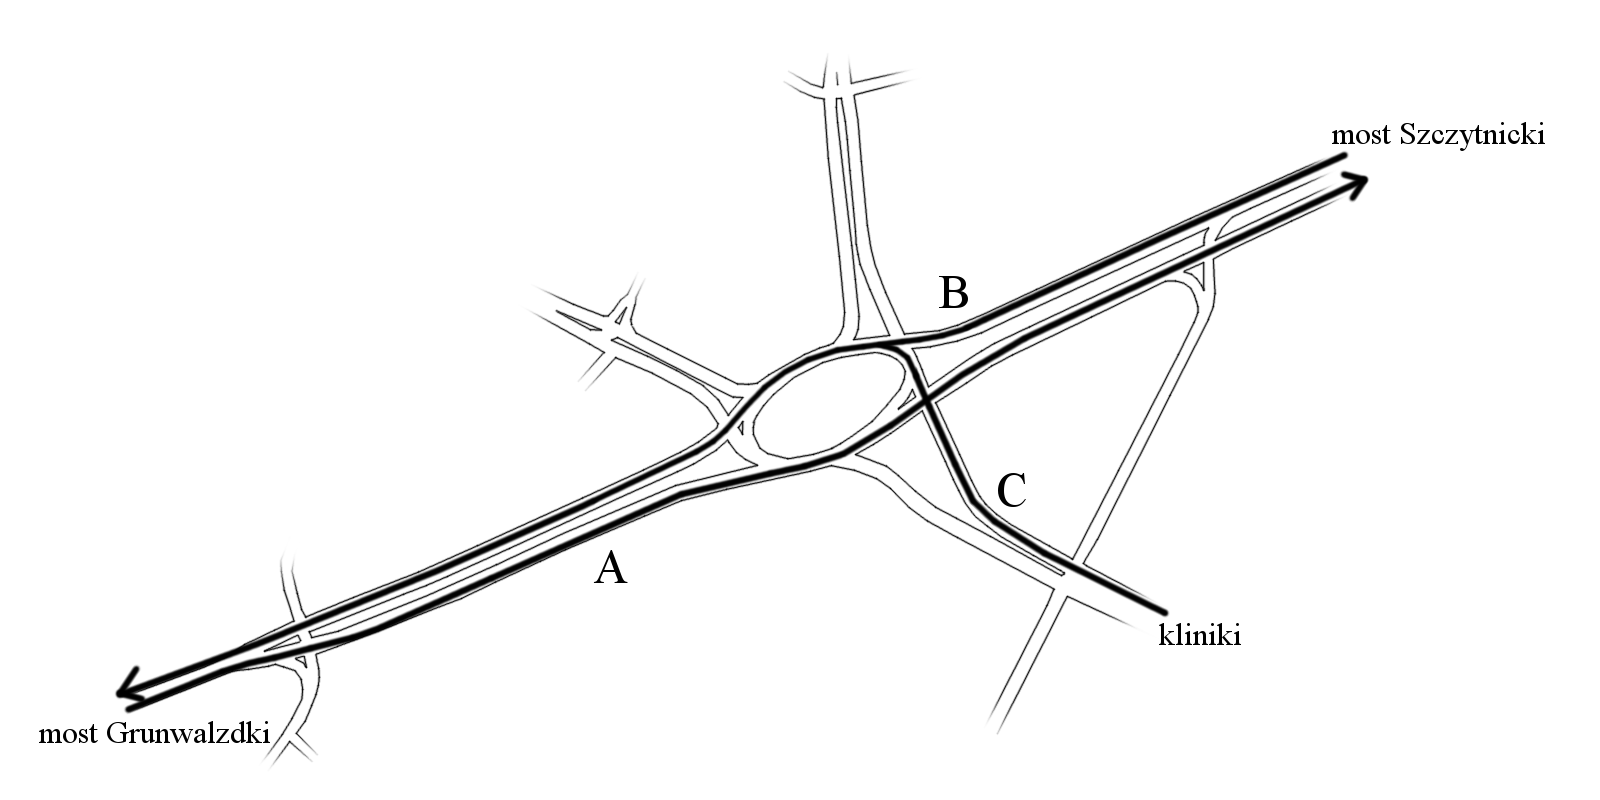
\includegraphics[width=1.0\textwidth]{images/mapa_trasy.png}
    \caption{Mapa przedstawiająca badane trasy przejazdu, przygotowana na podstawie Google Maps \cite{google_maps}}
    \label{fig:mapa_trasy}
\end{figure}
\FloatBarrier

W dalszej części badane były czasy przejazdu na trzech wybranych trasach, przedstawionych na rysunku \ref{fig:mapa_trasy}.
Trasa A, z mostu Grunwaldzkiego w kierunku mostu Szczytnickiego, oraz trasa B, z kierunku mostu Szczytnickiego do mostu Grunwaldzkiego jest wspomnianą wcześniej drogą główną, na której opóźnienia, w przypadku braku sterowania, powstają ze względu na tworzenie się korków. Trasa C z klinik (ulica Skłodowskiej-Curie) do mostu Grunwaldzkiego jest trasą podporządkowaną przez co ruch na niej zależy w dużym stopniu od ruchu na dwóch pozostałych trasach.

\FloatBarrier
\begin{figure}[h]
    \centering
    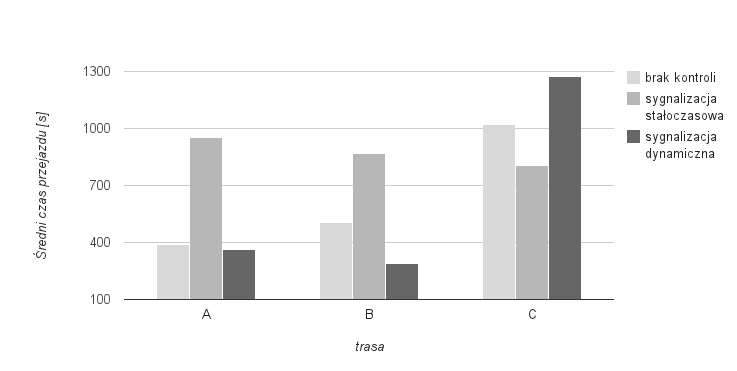
\includegraphics[width=1.0\textwidth]{images/wykres_typ_sterowania_czas.png}
    \caption{Wykres zależności średniego czasu przejazdu od typu sterowania}
    \label{fig:wykres_typ_sterowania_czas}
\end{figure}
\FloatBarrier
\begin{table}[h]
	\centering
	\begin{tabular}{ |r|c|c|c| }
		\hline
		& trasa A & trasa B & trasa C \\
		\hline
		brak kontroli & 389,58 s & 504,49 s & 1019,22 s \\
		\hline
		sygnalizacja stałoczasowa & 951,87 s & 867,70 s & 806,33 s \\
		\hline
		sygnalizacja dynamiczna & 365,05 s & 288,85 s & 1273,50 s \\
		\hline
	\end{tabular}
	\caption{Zależność średniego czasu przejazdu od typu sterowania}
	\label{tab:wykres_typ_sterowania_czas}
\end{table}
\FloatBarrier
Przedstawione na wykresie \ref{fig:wykres_typ_sterowania_czas} i w tabeli \ref{tab:wykres_typ_sterowania_czas} zmierzone średnie czasy przejazdu na wybranych trasach przedstawiają podstawowe róznice w sterowaniu stałoczasowym o stałym programi i sterowaniu dynamicznym. Sterowanie stałoczasowe charakteryzuje się wyrównaniem czasów przejazdu na wybranych trasach, co w przypadku trasy C pokazuje zdecydowaną poprawę.

Badany algorytm dynamiczny wykazuje poprawę w przypadku tras A i B, jednak powoduje również pogorszenie sytuacji dla trasy C. Może to być spowodowane metodą wyznaczania następnego stanu sterowania. Wyliczana jest suma wag poszczególnych sygnalizatorów. W dojeździe do punktu kolizji tras A i B z trasą C, trasa C posiada 3 sygnalizatory natomiast A i B posiadają 6 sygnalizatorów na niekolidujących strumieniach ruchu.

\FloatBarrier
\begin{figure}[h]
    \centering
    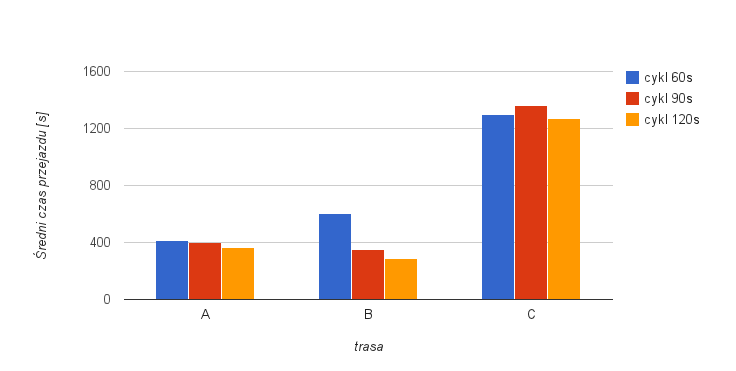
\includegraphics[width=1.0\textwidth]{images/wykres_dlugosc_cyklu_czas.png}
    \caption{Wykres zależności średniego czasu przejazdu od długości cyklu w sygnalizacji dynamicznej}
    \label{fig:wykres_dlugosc_cyklu_czas}
\end{figure}
\FloatBarrier
\begin{table}[h]
	\centering
	\begin{tabular}{ |r|c|c|c| }
		\hline
		& trasa A & trasa B & trasa C \\
		\hline
		cykl 60 s & 412,72 s & 602,86 s & 1301,70 s \\
		\hline
		cykl 90 s & 398,09 s & 353,62 s & 1361,07 s \\
		\hline
		cykl 120 s & 365,05 s & 288,85 s & 1273,50 s \\
		\hline
	\end{tabular}
	\caption{Zależność średniego czasu przejazdu od długości cyklu w sygnalizacji dynamicznej}
	\label{tab:wykres_dlugosc_cyklu_czas}
\end{table}
\FloatBarrier
Na wykresie \ref{fig:wykres_dlugosc_cyklu_czas} i w tabeli \ref{tab:wykres_dlugosc_cyklu_czas} widzimy zależność czasu przejazdu od długości cyklu. W tym przypadku, podobnie jak dla wartości średniej liczby zatrzymań i prędkości przedstawionych w tabeli \ref{tab:predkosc}, lepsze wyniki uzyskuje większa długość cyklu świetlnego.

\FloatBarrier
\begin{figure}[h]
    \centering
    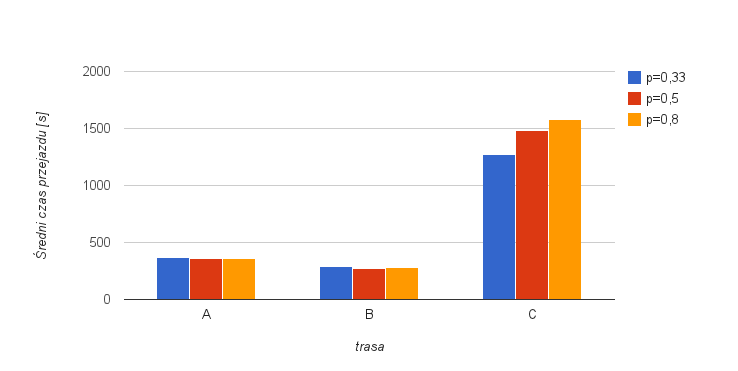
\includegraphics[width=1.0\textwidth]{images/wykres_przewidywany_przeplyw_czas.png}
    \caption{Wykres zależności średniego czasu przejazdu od wpływu przewidywanego przepływu na sterowanie (p) w sygnalizacji dynamicznej}
    \label{fig:wykres_przewidywany_przeplyw_czas}
\end{figure}
\FloatBarrier
\begin{table}[h]
	\centering
	\begin{tabular}{ |r|c|c|c| }
		\hline
		& trasa A & trasa B & trasa C \\
		\hline
		p=0,33 & 365,05 s & 288,85 s & 1273,50 s \\
		\hline
		p=0,5 & 356,70 s & 272,23 s & 1484,91 s \\
		\hline
		p=0,8 & 361,30 s & 279,42 s & 1581,82 s \\
		\hline
	\end{tabular}
	\caption{Zależność średniego czasu przejazdu od wpływu przewidywanego przepływu na sterowanie (p) w sygnalizacji dynamicznej}
	\label{tab:wykres_przewidywany_przeplyw_czas}
\end{table}
\FloatBarrier
Wykres \ref{fig:wykres_przewidywany_przeplyw_czas} i tabela \ref{tab:wykres_przewidywany_przeplyw_czas} przedstawia zależność wpływu przewidywanego przepływu na sterowanie. Widzimy że zwiększenie wielkości badanego parametru do wielkości q=0,5 powoduje poprawę czasu przejazdu dla tras A i B. Dalsze zwiększanie wielkości parametru zmienjsza efektywność. W przypadku trasy C można zaobserwować zwiększenie czasu przjazdu przy zwiększaniu wartości parametru.

\FloatBarrier
\begin{figure}[h]
    \centering
    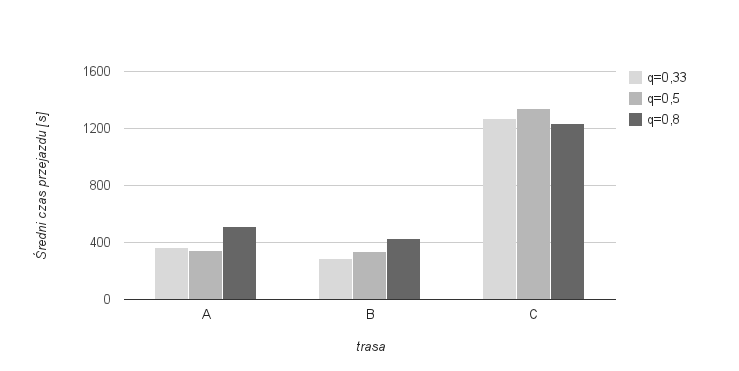
\includegraphics[width=1.0\textwidth]{images/wykres_przeplyw_czas.png}
    \caption{Wykres zależności średniego czasu przejazdu od wpływu aktualnego przepływu na sterowanie (q) w sygnalizacji dynamicznej}
    \label{fig:wykres_przeplyw_czas}
\end{figure}
\FloatBarrier
\begin{table}[h]
	\centering
	\begin{tabular}{ |r|c|c|c| }
		\hline
		& trasa A & trasa B & trasa C \\
		\hline
		q=0,33 & 365,05 s & 288,85 s & 1273,50 s \\
		\hline
		q=0,5 & 344,73 s & 337,45 s & 1341,16 s \\
		\hline
		q=0,8 & 511,69 s & 429,03 s & 1236,22 s \\
		\hline
	\end{tabular}
	\caption{Zależność średniego czasu przejazdu od wpływu aktualnego przepływu na sterowanie (q) w sygnalizacji dynamicznej}
	\label{tab:wykres_przeplyw_czas}
\end{table}
\FloatBarrier
Kolejny wykres (\ref{fig:wykres_przeplyw_czas}) przedstawia zależność czasu przejazdu od aktualnego przepływu pojazdów. W przypadku zwiększenia tego parametru możemy zaobserwować minimalną poprawę dla trasy A przy zmianie wielkości parametru na 0,5, przy dalszym zwiększaniu wartości parametru wynik pogarsza się.
Widać również pewną poprawę wyniku dla trasy C i wartości parametru 0,8.
Znaczenie tego parametru może być pomniejszone, przy wykonanych badaniach z wykorzystaniem dużego ruchu, ze względu na zmniejszenie przepływu w przypadku powstania korku. Zarówno pojazdy stojące w korku jak i brak pojazdów będzie odznaczał się wielkością przepływu 0 pojazdów na godzinę.

\FloatBarrier
\begin{figure}[h]
    \centering
    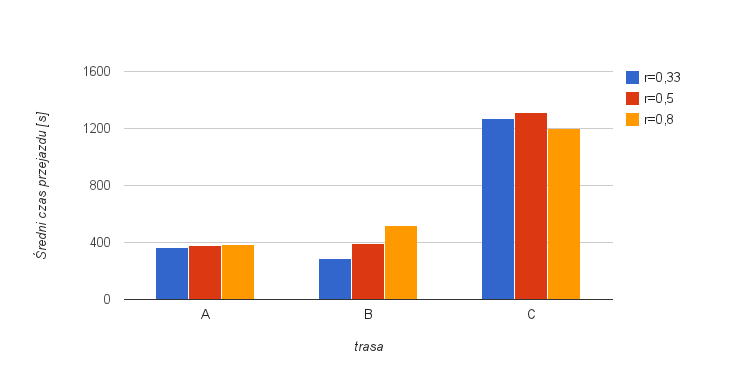
\includegraphics[width=1.0\textwidth]{images/wykres_kolejka_czas.png}
    \caption{Wykres zależności średniego czasu przejazdu od wpływu aktualnej kolejki na sterowanie (r) w sygnalizacji dynamicznej}
    \label{fig:wykres_kolejka_czas}
\end{figure}
\FloatBarrier
\begin{table}[h]
	\centering
	\begin{tabular}{ |r|c|c|c| }
		\hline
		& trasa A & trasa B & trasa C \\
		\hline
		r=0,33 & 365,05 s & 288,85 s & 1273,50 s \\
		\hline
		r=0,5 & 378,00 s & 392,09 s & 1314,89 s \\
		\hline
		r=0,8 & 385,92 s & 517,71 s & 1200,47 s \\
		\hline
	\end{tabular}
	\caption{Zależność średniego czasu przejazdu od wpływu aktualnej kolejki na sterowanie (r) w sygnalizacji dynamicznej}
	\label{tab:wykres_kolejka_czas}
\end{table}
\FloatBarrier
Na wykresie \ref{fig:wykres_kolejka_czas} i w tabeli \ref{tab:wykres_kolejka_czas} przedstawiona została zależność czasu przejazdu od wpływu aktualnej kolejki na sterowanie. Można zaobserwować, że zwiększenie wpływu kolejki na sterowanie powoduje zwiększenia czasu przejazdu na drodze głównej (trasach A i B). Jednocześnie dla wielkości parametru 0,8 czas przejazdu na trasie podporządkowanej zmniejszył się.
Podobnie jak w przypadku przepływu pojazdów, działanie tego parametru jest ograniczone. Znormalizowana wielkość kolejek będzie równa dla przeciążonej sieci drogowej